\iftrue % Déclaration sur l'honneur pour une thèse en français (inverser les \if pour une thèse en anglais)
    I, undersigned, Md Rasedujjaman, %% First Name and Surname of the PhD student
    hereby declare that the work presented in this manuscript is my own work, carried out under the scientific direction of Guillaume Maire and co-direction of Philippe Robert, %% First Name and Surname of the thesis director and if applicable of the co-thesis director
    in accordance with the principles of honesty, integrity and responsibility inherent to the research mission. The research work and the writing of this manuscript have been carried out in compliance with both the french national charter for Research Integrity and the Aix-Marseille University charter on the fight against plagiarism.
    
    This work has not been submitted previously either in this country or in another country in the same or in a similar version to any other examination body.\\
    
    Sylhet,  January 11, 2022
    
    \begin{flushright}
\includegraphics[width=120px,height=40px]{Signature_rased}\end{flushright}% signature
\fi

\iffalse % Affidavit of Honour for english thesis (invert the \if for an English thesis)
    I, undersigned, [First Name Surname], %% First Name and Surname of the PhD student
    hereby declare that the work presented in this manuscript is my own work, carried out under the scientific direction of [First Name Surname], %% First Name and Surname of the thesis director and if applicable of the co-thesis director
    in accordance with the principles of honesty, integrity and responsibility inherent to the research mission. The research work and the writing of this manuscript have been carried out in compliance with both the french national charter for Research Integrity and the Aix-Marseille University charter on the fight against plagiarism.
    
    This work has not been submitted previously either in this country or in another country in the same or in a similar version to any other examination body.\\
    
    [Place] [date]
    
    \begin{flushright}\includegraphics[width=120px,height=40px]{example-image-b}
\includegraphics[width=40,height=15px]{Signature_rased}\end{flushright} % signature
\fi

~\vfill
\begin{center}
	\begin{minipage}[c]{0.25\linewidth}
		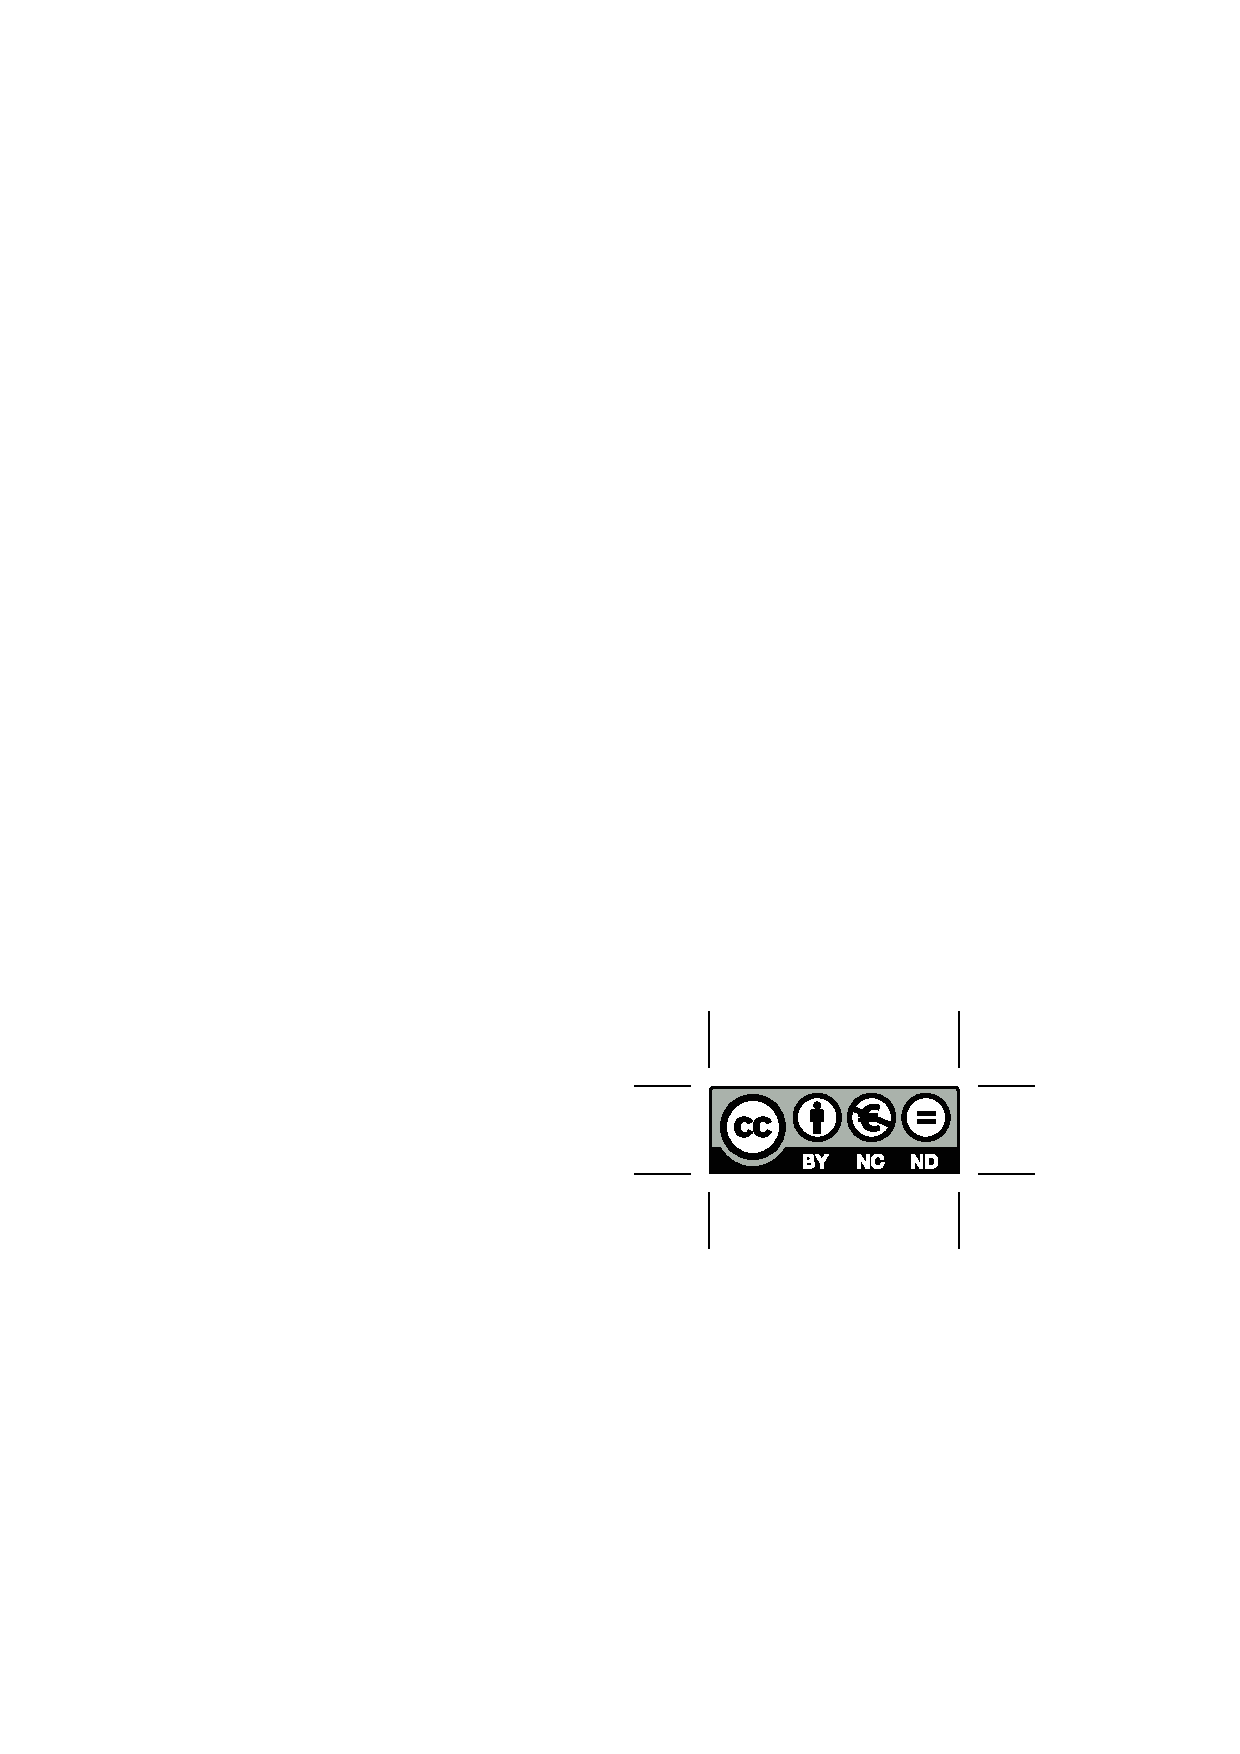
\includegraphics[height=35px]{by-nc-nd-eu}
	\end{minipage}\hfill
\end{center}

Cette \oe{}uvre est mise à disposition selon les termes de la \href{https://creativecommons.org/licenses/by-nc-nd/4.0/deed.fr}{Licence Creative Commons Attribution - Pas d’Utilisation Commerciale - Pas de Modification 4.0 International}. % consultez les conditions de la licence cc by-nc-nd, vous pouvez appliquer une licence moins restrictive, cc by-nc-sa par exemple
\newpage
